\mbox{$\displaystyle $\,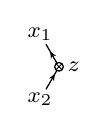
\begin{tikzpicture}[x=0.550cm, y=0.550cm, line width=0.450pt, baseline={([yshift=-0.6ex]0,0)}]
  \draw (0.000,0.000) -- (-0.300,0.520);
  \fill (-0.205,0.354) -- (-0.184,0.184) -- (-0.151,0.262) -- (-0.067,0.251) -- cycle;
  \draw (0.000,0.000) -- (-0.300,-0.520);
  \fill (-0.095,-0.165) -- (-0.233,-0.269) -- (-0.149,-0.258) -- (-0.116,-0.336) -- cycle;
  \draw[fill=white] (0.000,0.000) circle (0.100);
  \draw[line width=0.320pt] (0.070,0.070) -- (-0.070,-0.070) (0.070,-0.070) -- (-0.070,0.070);
  \node[font=\footnotesize, inner sep=0pt, anchor=180] at (0.190,0.000) {$z$};
  \node[font=\footnotesize, inner sep=0pt, anchor=300] at (-0.345,0.598) {$x_{1}$};
  \node[font=\footnotesize, inner sep=0pt, anchor=60] at (-0.345,-0.598) {$x_{2}$};
\end{tikzpicture}}
\diagramgap
\mbox{$\displaystyle +\,$\,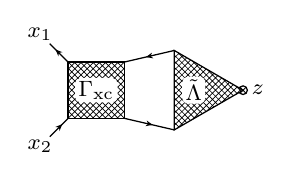
\begin{tikzpicture}[x=0.550cm, y=0.550cm, line width=0.450pt, baseline={([yshift=-0.6ex]0,0)}]
  \draw (-0.515,-0.650) -- (0.636,-0.917);
  \fill (0.137,-0.801) -- (-0.001,-0.700) -- (0.033,-0.777) -- (-0.032,-0.831) -- cycle;
  \draw (0.636,0.917) -- (-0.515,0.650);
  \fill (-0.017,0.765) -- (0.153,0.735) -- (0.087,0.790) -- (0.122,0.867) -- cycle;
  \draw (1.165,0.000) -- (0.636,0.917);
  \draw (1.165,0.000) -- (0.636,-0.917);
  \draw (1.165,0.000) -- (2.224,0.000);
  \draw (-1.165,0.000) -- (-1.815,0.650);
  \draw (-1.165,0.000) -- (-1.815,-0.650);
  \draw (-1.165,0.000) -- (-0.515,-0.650);
  \draw (-1.165,0.000) -- (-0.515,0.650);
  \draw (-1.815,0.650) -- (-2.239,1.074);
  \fill (-2.104,0.939) -- (-2.040,0.780) -- (-2.029,0.864) -- (-1.945,0.875) -- cycle;
  \draw (-1.815,-0.650) -- (-2.239,-1.074);
  \fill (-1.950,-0.785) -- (-2.110,-0.849) -- (-2.025,-0.860) -- (-2.014,-0.945) -- cycle;
  \draw[fill=white] (2.224,0.000) circle (0.100);
  \draw[line width=0.320pt] (2.294,0.070) -- (2.154,-0.070) (2.294,-0.070) -- (2.154,0.070);
  \fill[white] (0.636,0.917) -- (0.636,-0.917) -- (2.224,0.000) -- cycle;
  \draw[line width=0.248pt] (0.636,0.885) -- (0.656,0.905) (0.636,0.744) -- (0.746,0.853) (0.636,0.602) -- (0.835,0.802) (0.636,0.461) -- (0.925,0.750) (0.636,0.319) -- (1.014,0.698) (0.636,0.178) -- (1.104,0.646) (0.636,0.036) -- (1.194,0.594) (0.636,-0.105) -- (1.283,0.543) (0.636,-0.246) -- (1.373,0.491) (0.636,-0.388) -- (1.463,0.439) (0.636,-0.529) -- (1.552,0.387) (0.636,-0.671) -- (1.642,0.336) (0.636,-0.812) -- (1.732,0.284) (0.723,-0.866) -- (1.821,0.232) (1.057,-0.673) -- (1.911,0.180) (1.392,-0.480) -- (2.001,0.129) (1.727,-0.287) -- (2.090,0.077) (2.061,-0.094) -- (2.180,0.025) (0.636,-0.885) -- (0.656,-0.905) (0.636,-0.744) -- (0.746,-0.853) (0.636,-0.602) -- (0.835,-0.802) (0.636,-0.461) -- (0.925,-0.750) (0.636,-0.319) -- (1.014,-0.698) (0.636,-0.178) -- (1.104,-0.646) (0.636,-0.036) -- (1.194,-0.594) (0.636,0.105) -- (1.283,-0.543) (0.636,0.246) -- (1.373,-0.491) (0.636,0.388) -- (1.463,-0.439) (0.636,0.529) -- (1.552,-0.387) (0.636,0.671) -- (1.642,-0.336) (0.636,0.812) -- (1.732,-0.284) (0.723,0.866) -- (1.821,-0.232) (1.057,0.673) -- (1.911,-0.180) (1.392,0.480) -- (2.001,-0.129) (1.727,0.287) -- (2.090,-0.077) (2.061,0.094) -- (2.180,-0.025);
  \begin{scope}
  \clip (0.636,0.917) -- (0.636,-0.917) -- (2.224,0.000) -- cycle;
  \node[font=\footnotesize, inner sep=1.2pt, fill=white, rounded corners=2pt] at (1.085,0.000) {$\tilde\Lambda$};
  \end{scope}
  \draw (0.636,0.917) -- (0.636,-0.917) -- (2.224,0.000) -- cycle;
  \fill[white] (-1.815,-0.650) rectangle (-0.515,0.650);
  \draw[line width=0.248pt] (-1.815,0.481) -- (-1.646,0.650) (-1.815,0.340) -- (-1.505,0.650) (-1.815,0.199) -- (-1.364,0.650) (-1.815,0.057) -- (-1.222,0.650) (-1.815,-0.084) -- (-1.081,0.650) (-1.815,-0.226) -- (-0.939,0.650) (-1.815,-0.367) -- (-0.798,0.650) (-1.815,-0.509) -- (-0.656,0.650) (-1.815,-0.650) -- (-0.515,0.650) (-1.674,-0.650) -- (-0.515,0.509) (-1.532,-0.650) -- (-0.515,0.367) (-1.391,-0.650) -- (-0.515,0.226) (-1.249,-0.650) -- (-0.515,0.084) (-1.108,-0.650) -- (-0.515,-0.057) (-0.966,-0.650) -- (-0.515,-0.199) (-0.825,-0.650) -- (-0.515,-0.340) (-0.684,-0.650) -- (-0.515,-0.481) (-1.815,-0.481) -- (-1.646,-0.650) (-1.815,-0.340) -- (-1.505,-0.650) (-1.815,-0.199) -- (-1.364,-0.650) (-1.815,-0.057) -- (-1.222,-0.650) (-1.815,0.084) -- (-1.081,-0.650) (-1.815,0.226) -- (-0.939,-0.650) (-1.815,0.367) -- (-0.798,-0.650) (-1.815,0.509) -- (-0.656,-0.650) (-1.815,0.650) -- (-0.515,-0.650) (-1.674,0.650) -- (-0.515,-0.509) (-1.532,0.650) -- (-0.515,-0.367) (-1.391,0.650) -- (-0.515,-0.226) (-1.249,0.650) -- (-0.515,-0.084) (-1.108,0.650) -- (-0.515,0.057) (-0.966,0.650) -- (-0.515,0.199) (-0.825,0.650) -- (-0.515,0.340) (-0.684,0.650) -- (-0.515,0.481);
  \begin{scope}
  \clip (-1.815,-0.650) rectangle (-0.515,0.650);
  \node[font=\footnotesize, inner sep=1.2pt, fill=white, rounded corners=2pt] at (-1.165,0.000) {$\Gamma_{\rm xc}$};
  \end{scope}
  \draw (-1.815,-0.650) rectangle (-0.515,0.650);
  \node[font=\footnotesize, inner sep=0pt, anchor=180] at (2.414,0.000) {$z$};
  \node[font=\footnotesize, inner sep=0pt, anchor=315] at (-2.303,1.138) {$x_{1}$};
  \node[font=\footnotesize, inner sep=0pt, anchor=45] at (-2.303,-1.138) {$x_{2}$};
\end{tikzpicture}}
